\subsection{Cifrado Feistel}

Consiste en un \gls{gl:cifrado_iterativo} que mapea bloques de 
texto en claro de tamaño $2t$bits (separados en bloques 
$L_0, R_0$ de tamaño $t$) a un texto cifrado $R_r$, $L_r$
mediante un proceso de $r$ \glspl{gl:ronda}. 

\begin{pseudocodigo}[caption={Feistel, cifrado.}, label={feistel:1}]
  inicio
  para_todo $i$ desde 1 hasta $r$: 
    $L_i = R_{i-1}$
    $R_i = L_{i-1} \oplus f(R_{i-1}, K_i)$
  fin
  fin
\end{pseudocodigo}
Donde cada subllave $K_i$ se obtiene de la llave $K$.

Normalmente el número de rondas $r$ es mayor o igual a tres y par. 
Además, casi siempre intercambia el orden de los bloques de salida al 
revés en la última ronda: ($R_r, L_r$) en vez de ($L_r, R_r$). 

El descifrado se realiza utilizando el mismo proceso de cifrado pero 
con las llaves en el orden inverso (comenzando con $K_r$ hasta $K_1$).

\begin{figure}[H]
  \begin{center}
    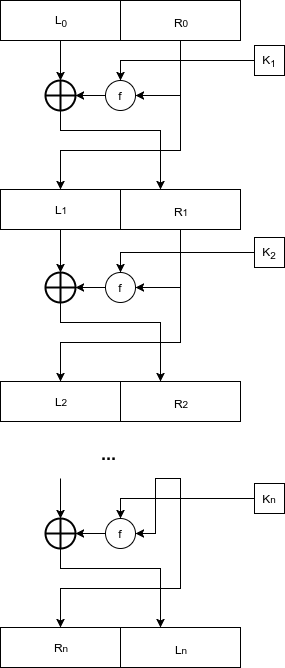
\includegraphics[width=0.4\linewidth]
      {contenidos/antecedentes/bloques/diagramas/feistel}
     \caption{Diagrama genérico de una red Feistel.}
   \end{center}
\end{figure}